%%%%%%%%%%%%%%%%%%%%%%%%%%%%%%%%%%%%%%%%%%%%%%%%%%%%%%%%%%%%%%%%%%%%%%%%%%%%%%%%
%                    Capitulo 8: Experimentacion                               %
%%%%%%%%%%%%%%%%%%%%%%%%%%%%%%%%%%%%%%%%%%%%%%%%%%%%%%%%%%%%%%%%%%%%%%%%%%%%%%%%

\chapter{Experimentación}

Una vez que el sistema ha sido implementado y validado, es necesario realizar un estudio
de su funcionamiento. Este estudio consiste en llevar a cabo una serie de experimentos,
los cuales pretenden poner a prueba dos aspectos fundamentales del sistema:

\begin{enumerate}
    \item La capacidad que tiene para generar problemas \texttt{PDDL} de forma
    automática a partir de los estados del juego.
    \item La capacidad que tiene para responder a los cambios dinámicos que
    se producen en los juegos.
\end{enumerate}

Para llevar a cabo estos experimentos se han escogido los siguientes juegos:

% Comentar aquí los juegos, relacionandolos con las imagenes
\begin{itemize}[label=\textbullet]
    \item \textbf{\textit{Boulderdash}}. El objetivo del juego consiste en recoger 9 de
    las gemas que hay esparcidas a lo largo de todo el mapa y llegar hasta la salida,
    esquivando a los enemigos (escorpiones y mariposas)
    
    \item \textbf{\textit{Ice and Fire}}.
    
    \item \textbf{\textit{Labyrinth Dual}}.
\end{itemize}

\begin{figure}[H]
    \centering
    \begin{subfigure}[t]{.5\textwidth}
        \centering
        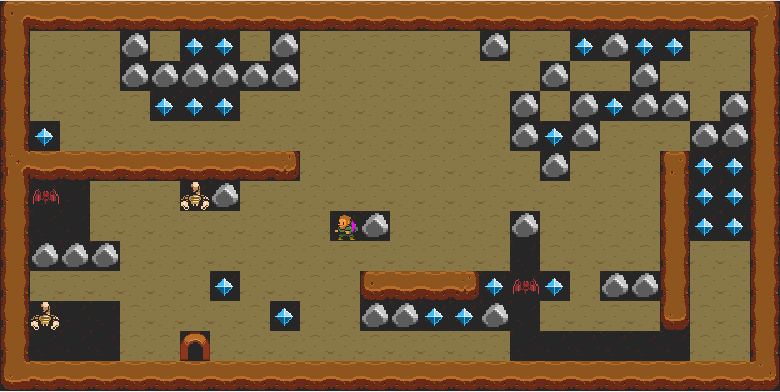
\includegraphics[scale=0.3]{img/CH08/boulderdash.png}
        \caption{\textit{Boulderdash}.}
        \label{fig:boulderdash}
    \end{subfigure}%
    \begin{subfigure}[t]{.5\textwidth}
        \centering
        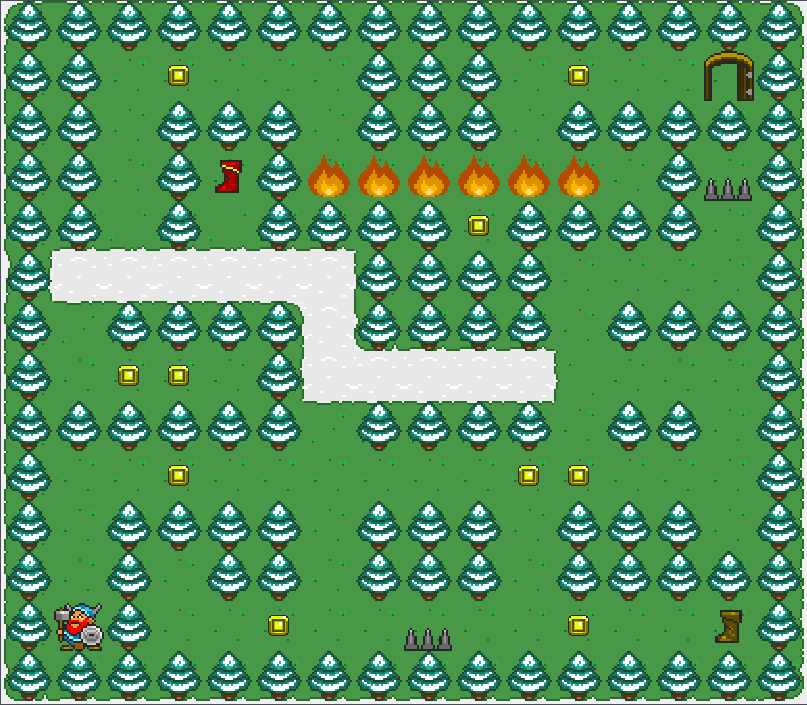
\includegraphics[scale=0.25]{img/CH08/ice_and_fire.png}
        \caption{\textit{Ice and Fire}.}
        \label{fig:ice_and_fire}
    \end{subfigure}
    \par\bigskip
    \begin{subfigure}[t]{0.5\textwidth}
        \centering
        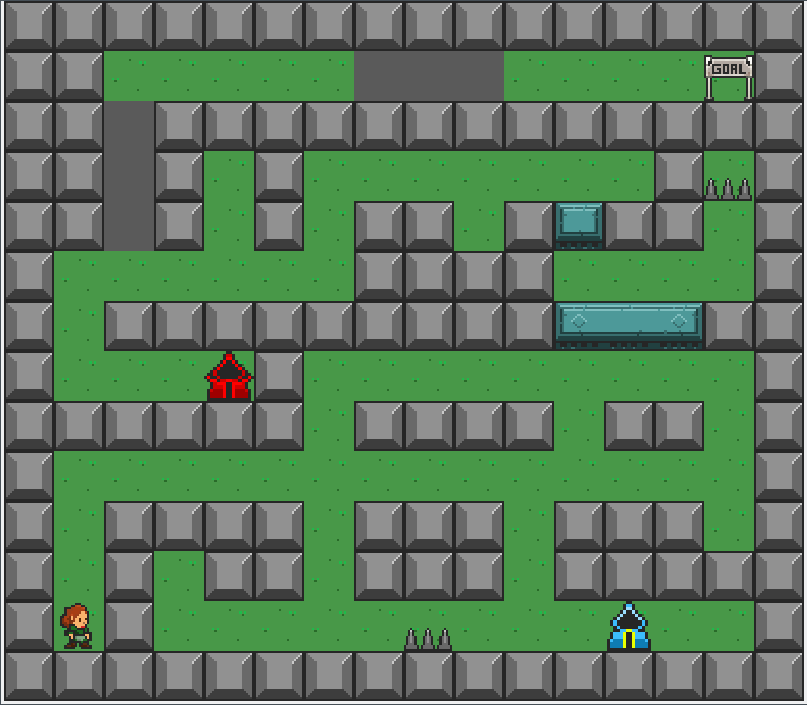
\includegraphics[scale=0.25]{img/CH08/labyrinth_dual.png}
        \caption{\textit{Labyrinth Dual}.}
        \label{fig:labyrinth_dual}
    \end{subfigure}
    \caption{Juegos con los que se han realizado los experimentos.}
    \label{fig:games}
\end{figure}

% Comentar los dominios creados

\begin{table}[H]
\centering
\begin{tabular}{|c|ccc|}
\hline
\textbf{Juego} & \textbf{Predicados} & \textbf{Tipos} & \textbf{Acciones} \\ \hline
\textit{Boulderdash} & 15 & 9 & 17 \\ \hline
\textit{Ice and Fire} & 13 & 10 & 14 \\ \hline
\textit{Labyrinth Dual} & 12 & 9 & 14 \\ \hline
\end{tabular}
\caption{Información sobre los dominios creados para cada juego.}
\label{tab:info-domains}
\end{table}

% Explicar que se han cambiado algunos parametros del entorno

\section{Generación de problemas}

% Comentar experimentacion llevada a cabo y resultados por encima, diciendo que
% si no se usase este sistema la generación manual podría tardar días/semanas

\begin{landscape}
\begin{table}[]
\centering
\resizebox{1.5\textwidth}{!}{%
\begin{tabular}{|c|c|cccccccc|}
\hline
\textbf{Juego} &
  \textbf{Nivel} &
  \textbf{Objetivos} &
  \textbf{\begin{tabular}[c]{@{}c@{}}Predicados problema\\ inicial\end{tabular}} &
  \textbf{\begin{tabular}[c]{@{}c@{}}Objetos problema\\ inicial\end{tabular}} &
  \textbf{\begin{tabular}[c]{@{}c@{}}Tiempo medio\\ ejecución (s)\end{tabular}} &
  \textbf{\begin{tabular}[c]{@{}c@{}}Tiempo medio\\ predicados\\ conectividad (s)\end{tabular}} &
  \textbf{\begin{tabular}[c]{@{}c@{}}Tiempo medio\\ traducción estado\\ de observación (s)\end{tabular}} &
  \textbf{\begin{tabular}[c]{@{}c@{}}Tiempo medio\\ generación archivo\\ de problema (s)\end{tabular}} &
  \textbf{\begin{tabular}[c]{@{}c@{}}Tiempo medio total\\ generación problema\\ (s)\end{tabular}} \\ \hline
\multirow{5}{*}{\textit{Boulderdash}}    & \textbf{0} & 10 & 1735 & 400 & 0.4967 & 0.0313 & 0.0024 & 0.0038 & 0.0375 \\ \cline{2-10} 
                                         & \textbf{1} & 10 & 1721 & 393 & 0.428  & 0.0323 & 0.0029 & 0.0039 & 0.0392 \\ \cline{2-10} 
                                         & \textbf{2} & 10 & 1717 & 391 & 0.5293 & 0.0347 & 0.0034 & 0.0044 & 0.0425 \\ \cline{2-10} 
                                         & \textbf{3} & 10 & 1733 & 399 & 0.7487 & 0.0327 & 0.0049 & 0.0048 & 0.0423 \\ \cline{2-10} 
                                         & \textbf{4} & 10 & 1731 & 398 & 0.4403 & 0.0317 & 0.0030 & 0.0039 & 0.0386 \\ \hline
\multirow{5}{*}{\textit{Ice and Fire}}   & \textbf{0} & 3  & 1215 & 391 & 0.417  & 0.027  & 0.0026 & 0.003  & 0.0326 \\ \cline{2-10} 
                                         & \textbf{1} & 3  & 1234 & 410 & 0.4827 & 0.0307 & 0.0028 & 0.0056 & 0.0390 \\ \cline{2-10} 
                                         & \textbf{2} & 3  & 1235 & 411 & 0.522  & 0.0273 & 0.0031 & 0.0045 & 0.0349 \\ \cline{2-10} 
                                         & \textbf{3} & 3  & 1219 & 395 & 0.4587 & 0.0323 & 0.0029 & 0.0061 & 0.0413 \\ \cline{2-10} 
                                         & \textbf{4} & 3  & 1210 & 386 & 0.697  & 0.0273 & 0.0031 & 0.0055 & 0.0359 \\ \hline
\multirow{5}{*}{\textit{Labyrinth Dual}} & \textbf{0} & 3  & 1085 & 369 & 0.4503 & 0.0303 & 0.0029 & 0.0043 & 0.0376 \\ \cline{2-10} 
                                         & \textbf{1} & 2  & 1069 & 380 & 0.3847 & 0.0303 & 0.0027 & 0.0045 & 0.0376 \\ \cline{2-10} 
                                         & \textbf{2} & 3  & 1073 & 378 & 0.4107 & 0.0287 & 0.0024 & 0.0029 & 0,0339 \\ \cline{2-10} 
                                         & \textbf{3} & 3  & 1083 & 376 & 0.41   & 0.0297 & 0.0031 & 0.0052 & 0.038  \\ \cline{2-10} 
                                         & \textbf{4} & 2  & 1079 & 363 & 0.5623 & 0.029  & 0.0029 & 0.0062 & 0.0381 \\ \hline
\end{tabular}%
}
\caption{Resultados de la experimentación.}
\label{tab:exp-results}
\end{table}
\end{landscape}

\section{Respuesta a cambios dinámicos}

% Comentar brevemente qué se ha hecho

\begin{figure}[H]
    \centering
    \begin{subfigure}{\textwidth}
        \centering
        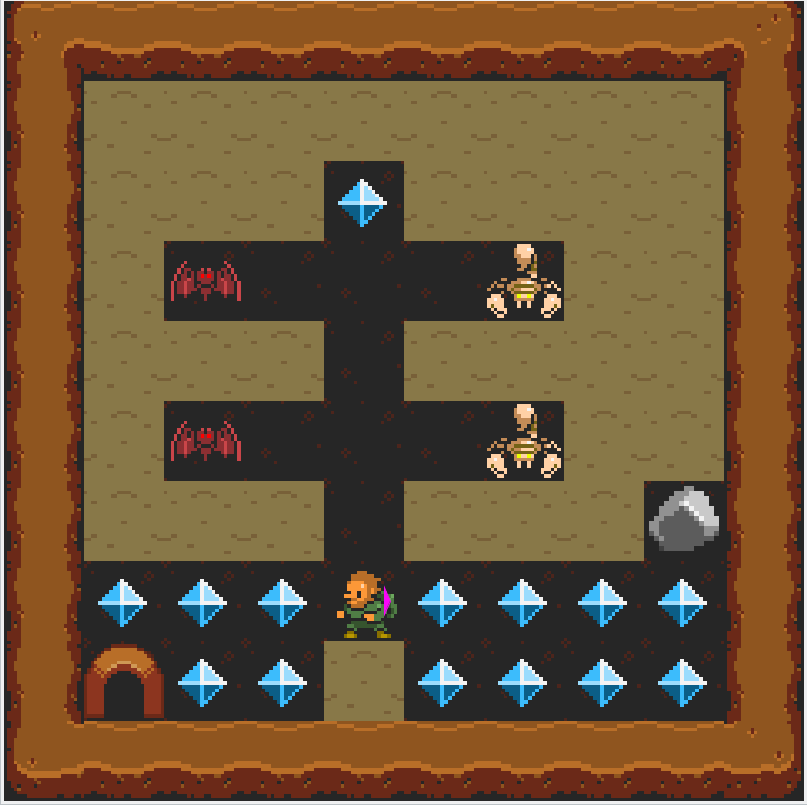
\includegraphics[scale=0.25]{img/CH08/discrepancy_1.png}
        \caption{Estado inicial del juego.}
        \label{fig:discrepancy_1}
    \end{subfigure}
    \par\bigskip
    \begin{subfigure}{\textwidth}
        \centering
        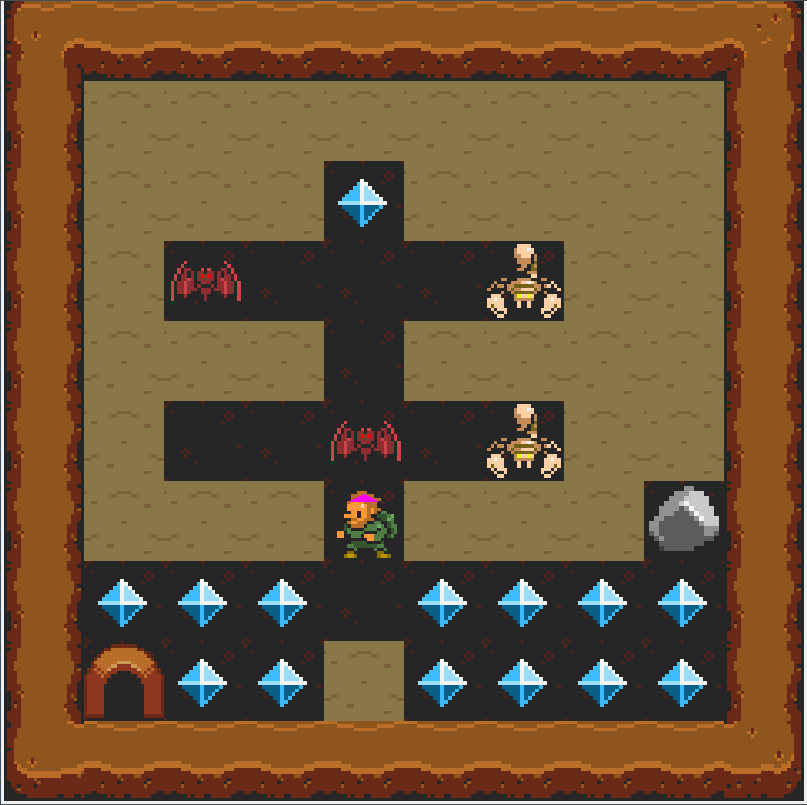
\includegraphics[scale=0.25]{img/CH08/discrepancy_2.png}
        \caption{Mariposa bloquea el camino.}
        \label{fig:discrepancy_2}
    \end{subfigure}
    \par\bigskip
    \begin{subfigure}{\textwidth}
        \centering
        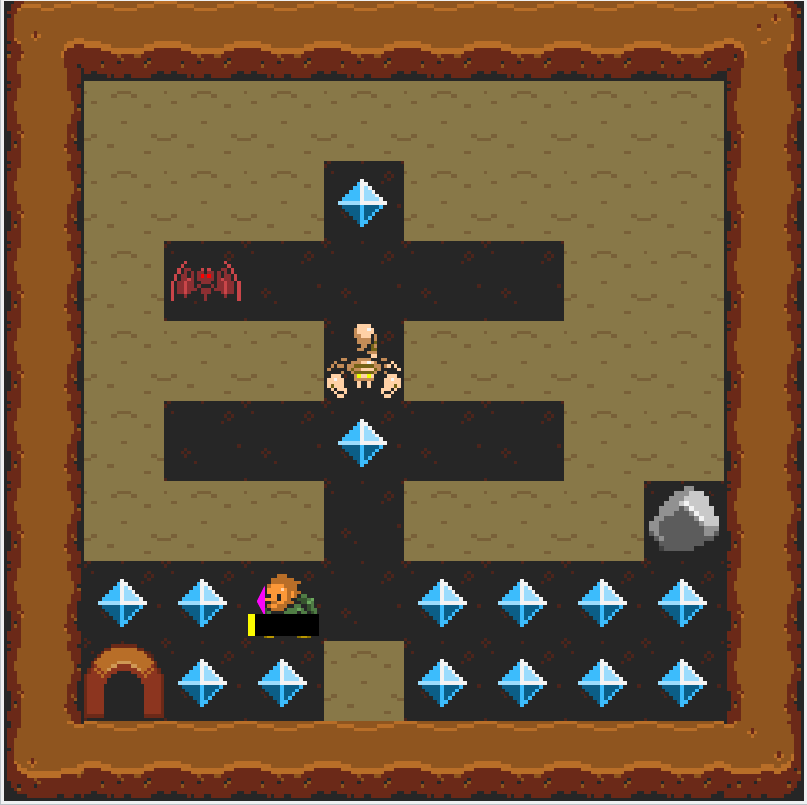
\includegraphics[scale=0.25]{img/CH08/discrepancy_3.png}
        \caption{Agente cambia de objetivo y lo alcanza.}
        \label{fig:discrepancy_3}
    \end{subfigure}
    \caption{Ejemplo de respuesta a cambios dinámicos en el entorno.}
    \label{fig:discrepancies}
\end{figure}